
\documentclass[hyperref={pdfpagelabels=false},ngerman]{beamer}

% stop font warning
\let\Tiny=\tiny
\providecommand\thispdfpagelabel[1]{}

\usepackage[english]{babel}
\usepackage{lmodern}
\usepackage[T1]{fontenc}
\usepackage[utf8]{inputenc}
\usepackage{graphicx,import}
\usepackage{feynmp}
\DeclareGraphicsRule{*}{mps}{*}{} 
\DeclareGraphicsExtensions{.pdf}
\usepackage{amsmath,amssymb,amstext,amsfonts,ulem} % mathrsfs
\usepackage{array,booktabs,tabularx}
\usepackage{tikz,tikz-uml,pgf-pie}
\usetikzlibrary{shapes,calc,arrows,positioning}
\tikzstyle{block} = [rectangle, draw, text width=7em, text centered, minimum height=2em]
\tikzstyle{arrow} = [draw, -latex, thick]
\tikzstyle{arrow2} = [draw, latex-latex, thick]
\tikzstyle{quark}  = [rectangle, draw, fill=yellow, minimum width=2em, text centered, minimum height=2em]
\tikzstyle{lepton} = [rectangle, draw, fill=red!50, minimum width=2em, text centered, minimum height=2em]
\tikzstyle{gauge}  = [circle   , draw, fill=green , minimum size=2em, inner sep=0pt, text centered]
\tikzstyle{scalar} = [diamond  , draw, fill=blue!40, minimum width=2.3em, text centered, minimum height=2.3em, inner sep=0pt]
\tikzstyle{goldstone} = [diamond, draw, dashed, fill=blue!30, minimum width=2.3em, text centered, minimum height=2.3em, inner sep=0pt]
\tikzstyle{squark}   = [diamond, draw, fill=yellow, minimum width=2.3em, text centered, minimum height=2.3em, inner sep=0pt]
\tikzstyle{slepton}  = [diamond, draw, fill=red!50, minimum width=2.3em, text centered, minimum height=2.3em, inner sep=0pt]
\tikzstyle{gaugino}  = [rectangle, draw, fill=green , minimum size=2em, inner sep=0pt, text centered]
\tikzstyle{higgsino} = [rectangle, draw, fill=blue!40  , minimum width=2em, text centered, minimum height=2em]
\tikzstyle{inert}    = [diamond  , draw, fill=teal!80, minimum width=2.3em, text centered, minimum height=2.3em, inner sep=0pt]
\tikzstyle{inertino} = [rectangle, draw, fill=teal!80, minimum width=2em, text centered, minimum height=2em]
\tikzstyle{phantom}  = [rectangle, minimum width=2em, text centered, minimum height=2em]
\usepackage{slashed}
\usepackage{fixltx2e} % textsubscript
\usepackage{multirow}
\usepackage{tcolorbox}
\usepackage{pifont}
\usepackage{xspace}
\usepackage{hyperref}
\hypersetup{colorlinks,linkcolor=,urlcolor=blue}
\usepackage{listings}
\lstset{breaklines=true,
  breakatwhitespace=true,
%  numbers=left,
  numberstyle=\tiny,
  stepnumber=1,
  basicstyle=\ttfamily\footnotesize,
  commentstyle=\ttfamily\color{gray},
  postbreak={\mbox{{$\hookrightarrow$}}\space\space},
  breakindent=10pt,
  breakautoindent=false,
  showspaces=false,
  showstringspaces=false,
  frame=single}

\definecolor{darkgreen}{RGB}{0,176,0}

\newcommand{\cmark}{\ding{51}}%
\newcommand{\xmark}{\ding{55}}%
\newcommand{\fmfvcenter}[1]{\;\vcenter{\hbox{\fmfreuse{#1}}}\;}
\newcommand{\eh}[1]{\,\mathsf{#1}}
\newcommand{\MeV}{\eh{MeV}}
\newcommand{\GeV}{\eh{GeV}}
\newcommand{\TeV}{\eh{TeV}}
\newcommand{\ok}{\textcolor{darkgreen}{\cmark}}
\newcommand{\notok}{\textcolor{red}{\xmark}}
\newcommand{\maybe}{\textcolor{gray}{\cmark}}
\newcommand{\meh}{\textcolor{gray}{\textbf{\huge\lower.1em\hbox{-}}}}
\newcommand{\Lagr}{\mathcal{L}}
\newcommand{\MS}{\ensuremath{M_S}}
\newcommand{\mathi}{\mathsf{i}}
\newcommand{\mycite}[1]{\ensuremath{\text{\textcolor{darkgray}{\tiny [#1]}}}}
\newcommand{\bigcite}[1]{\textcolor{darkgray}{[#1]}}
\newcommand{\dimrep}[1]{\mathbf{#1}}
\newcommand{\dimrepadj}[1]{\mathbf{\overline{#1}}}
\newcommand{\ESSM}{E\textsubscript{6}SSM}
\newcommand{\CESSM}{CE\textsubscript{6}SSM}
\DeclareMathOperator{\tildeRe}{\widetilde Re}
\DeclareMathOperator{\sign}{sign}
\DeclareMathOperator{\re}{Re}
\DeclareMathOperator{\im}{Im}
\renewcommand{\emph}{\textbf}
\newcommand{\dd}{\mathsf{d}}
\newcommand{\myurl}[1]{\href{#1}{#1}}
\newcommand{\Superpot}{\mathcal{W}}
\newcommand{\SuperField}[1]{#1}
\newcommand{\ConjSuperField}[1]{\bar{#1}}
\newcommand{\UY}{\ensuremath{U(1)_{Y}}}
\newcommand{\UN}{\ensuremath{U(1)_{N}}}
\newcommand{\Uem}{\ensuremath{U(1)_\text{em}}}
\newcommand{\SUL}{\ensuremath{SU(2)_\text{L}}}
\newcommand{\SUc}{\ensuremath{SU(3)_\text{c}}}
\newcommand{\SOten}{\ensuremath{{SO(10)}}}
\newcommand{\comma}{,}
\newcommand{\DRbar}{\ensuremath{\overline{\text{DR}}}}
\newcommand{\MSbar}{\ensuremath{\overline{\text{MS}}}}
\newcommand{\SM}{\ensuremath{\text{SM}}}
\newcommand{\MSSM}{\ensuremath{\text{MSSM}}}
\newcommand{\pole}{\ensuremath{\text{pole}}}
\newcommand{\match}{\ensuremath{\text{match}}}
\newcommand{\tree}{\ensuremath{\text{tree}}}
\newcommand{\fsstar}{\textbf{*}}
\newcommand{\fs}{\texttt{FlexibleSUSY}\xspace}
\newcommand{\fsh}{\texttt{FS+H}\xspace}
\newcommand{\feft}{\texttt{FlexibleEFTHiggs}\xspace}
\newcommand{\hssusy}{\texttt{HSSUSY}\xspace}
\newcommand{\Himalaya}{\texttt{Himalaya}\xspace}
\newcommand{\FH}{\texttt{FeynHiggs}\xspace}
\newcommand{\SPheno}{\texttt{SPheno}\xspace}
\newcommand{\SARAH}{\texttt{SARAH}\xspace}
\newcommand{\Zv}{\ensuremath{\backslash\mkern-11.0mu{Z_3}}}
\newcommand{\downrightknickarrow}{\mathrel{\scalebox{1.3}{\rotatebox[origin=c]{180}{$\Lsh$}}}}
\newcommand{\threelinebrace}{$\left. \begin{array}{c} \\ \\ \\ \end{array} \right\rbrace$}
\newcommand{\fivelinebrace}{$\left. \begin{array}{c} \\ \\ \\ \\ \\ \end{array} \right\rbrace$}
\newcommand{\twolinebrace}{$\left. \begin{array}{c} \\ \\ \end{array} \right\rbrace$}
\newcommand{\elevenlinebrace}{$\left. \begin{array}{c} \\ \\ \\ \\ \\ \\ \\ \\ \\ \\ \\ \end{array} \right\rbrace$}
\newcommand{\at}{\alpha_t}
\newcommand{\ab}{\alpha_b}
\newcommand{\atau}{\alpha_\tau}
\newcommand{\as}{\alpha_s}
\newcommand{\aem}{\alpha_\text{em}}
\newcommand{\Loop}{\ensuremath{\ell}\xspace}
\newcommand{\avnote}[1]{\textcolor{blue}{[#1]}}
\DeclareMathOperator{\Eigenvalue}{Eigenvalue}
\newcommand{\SQCD}{\ensuremath{\scalefont{.8}\text{SQCD}}}
\newcommand{\Qpole}{\ensuremath{Q_\text{pole}}}
\newcommand{\Qmatch}{\ensuremath{Q_\text{match}}}
\newcommand{\DMh}{\ensuremath{\Delta M_h^{(\texttt{SS+H})}}}
\newcommand{\DMhQpole}{\ensuremath{\Delta M_h^{(\Qpole)}}}
\newcommand{\DMhQmatch}{\ensuremath{\Delta M_h^{(\Qmatch)}}}
\newcommand{\DMhMt}{\ensuremath{\Delta M_h^{(m_t)}}}
\newcommand{\DMhAlphaS}{\ensuremath{\Delta M_h^{(\as)}}}
\newcommand{\DMhAlphaEm}{\ensuremath{\Delta M_h^{(\aem)}}}
\newcommand{\DMhHSSUSY}{\ensuremath{\Delta M_h^{(\HSSUSY)}}}
\newcommand{\DMhHSSUSYytSM}{\ensuremath{\Delta M_h^{(y_t^\SM)}}}
\newcommand{\DMhHSSUSYytMSSM}{\ensuremath{\Delta M_h^{(y_t^\MSSM)}}}
\newcommand{\DMhEFT}{\ensuremath{\Delta M_h^{(v^2/\MS^2)}}}
\def\HSSUSY{\texttt{HSSUSY}}
\def\SUSYHD{\texttt{SusyHD}}

% set look of slides
\usetheme{Madrid}
\useoutertheme{default}
\useinnertheme{circles}
\usecolortheme{default}
\beamertemplatenavigationsymbolsempty % keine Navigationselemente
\setbeamersize{text margin left = 1cm, text margin right = 1cm}

% define footer
\makeatletter
\setbeamertemplate{footline}
{
  \hfill\hbox{\insertframenumber{} / \inserttotalframenumber\hspace*{4pt}}%
  \vskip3pt%
}
\makeatother
\usecolortheme{tud}

\title{Update on the Standard Model Uncertainty}

\author[Alexander Voigt]{Harun Acaroglu, \underline{Alexander Voigt}}

\date{KUTS-10 Dresden\\[1em] 08--10/04/2019}

% \institute[Aachen]{RWTH Aachen}
\subject{FlexibleSUSY,MSSM,Higgs,EFT}
\keywords{FlexibleSUSY,MSSM,Higgs,EFT}

%%%%%%%%%%%%%%%%%%%%%%%%%%%%%%%%%%%%%%%%%%%%%%%%%%%%%%%%%%%%%%%%%%%%%%%%%%%%%

\begin{document}

%%%%%%%%%%%%%%%%%%%%%%%%%%%%%%%%%%%%%%%%%%%%%%%%%%%%%%%%%%%%%%%%%%%%%%%%%%%%%

% Savebox which contains the the Feynman rules
\newsavebox{\feynmanrules}
\sbox{\feynmanrules}{
\begin{fmffile}{Feynman/higgs} % file name and path
  \fmfset{thin}{.8pt}
  \fmfset{wiggly_len}{5mm}
  \fmfset{dash_len}{2.5mm}
  \fmfset{dot_size}{1thick}
  \fmfset{arrow_len}{2.5mm}
  \fmfset{curly_len}{2.5mm}

\begin{fmfgraph*}(60,60)
  \fmfkeep{hX}
  \fmfleft{v1}
  \fmfright{v2}
  \fmf{higgs}{v1,c1}
  \fmf{higgs}{c2,v2}
  \fmf{quark,left,tension=0.5,label=$X$}{c1,c2}
  \fmf{quark,left,tension=0.5}{c2,c1}
\end{fmfgraph*}

\begin{fmfgraph*}(60,60)
  \fmfkeep{htop}
  \fmfleft{v1}
  \fmfright{v2}
  \fmf{higgs}{v1,c1}
  \fmf{higgs}{c2,v2}
  \fmf{quark,left,tension=0.5,label=$t$}{c1,c2}
  \fmf{quark,left,tension=0.5}{c2,c1}
\end{fmfgraph*}

\begin{fmfgraph*}(60,60)
  \fmfkeep{hstop}
  \fmfleft{v1}
  \fmfright{v2}
  \fmf{higgs}{v1,c1}
  \fmf{higgs}{c2,v2}
  \fmf{scalar,left,tension=0.5,label=$\tilde{t}_i$}{c1,c2}
  \fmf{scalar,left,tension=0.5}{c2,c1}
\end{fmfgraph*}

\begin{fmfgraph*}(60,60)
  \fmfkeep{hstopA}
  \fmfleft{v1}
  \fmfright{v2}
  \fmf{higgs}{v1,c,v2}
  \fmf{scalar,right,tension=0.8,label=$\tilde{t}_i$}{c,c}
\end{fmfgraph*}

\begin{fmfgraph*}(60,60)
  \fmfkeep{htoptad}
  \fmfleft{v1}
  \fmfright{v2}
  \fmftop{t1}
  \fmf{higgs}{v1,c,v2}
  \fmffreeze
  \fmf{higgs}{c,c1}
  \fmf{quark,right,tension=0.3,label=$t$}{c1,c2}
  \fmf{quark,right,tension=0.3}{c2,c1}
  \fmf{phantom,tension=10}{c2,t1}
\end{fmfgraph*}

\begin{fmfgraph*}(60,60)
  \fmfkeep{hstoptad}
  \fmfleft{v1}
  \fmfright{v2}
  \fmftop{t1}
  \fmf{higgs}{v1,c,v2}
  \fmffreeze
  \fmf{higgs}{c,c1}
  \fmf{scalar,right,tension=0.3,label=$\tilde{t}_i$}{c1,c2}
  \fmf{scalar,right,tension=0.3}{c2,c1}
  \fmf{phantom,tension=10}{c2,t1}
\end{fmfgraph*}
\end{fmffile}
}

%%%%%%%%%%%%%%%%%%%%%%%%%%%%%%%%%%%%%%%%
\begin{frame}[plain]
  \tikz [remember picture,overlay]
  \node at
    ([yshift=1.3cm,xshift=4cm]current page.south)
    {\includegraphics[height=2cm]{images/RWTH_Logo}};
  \titlepage  
\end{frame}

%%%%%%%%%%%%%%%%%%%%%%%%%%%%%%%%%%%%%%%%
\begin{frame}{Contents}
  \tableofcontents
\end{frame}

\section{Motivation}

%%%%%%%%%%%%%%%%%%%%%%%%%%%%%%%%%%%%%%%%
\begin{frame}{Contents}
  \tableofcontents[currentsection]
\end{frame}
%%%%%%%%%%%%%%%%%%%%%%%%%%%%%%%%%%%%%%%%

\begin{frame}{Motivation --- SM uncertainty in \SUSYHD}
  \begin{center}
    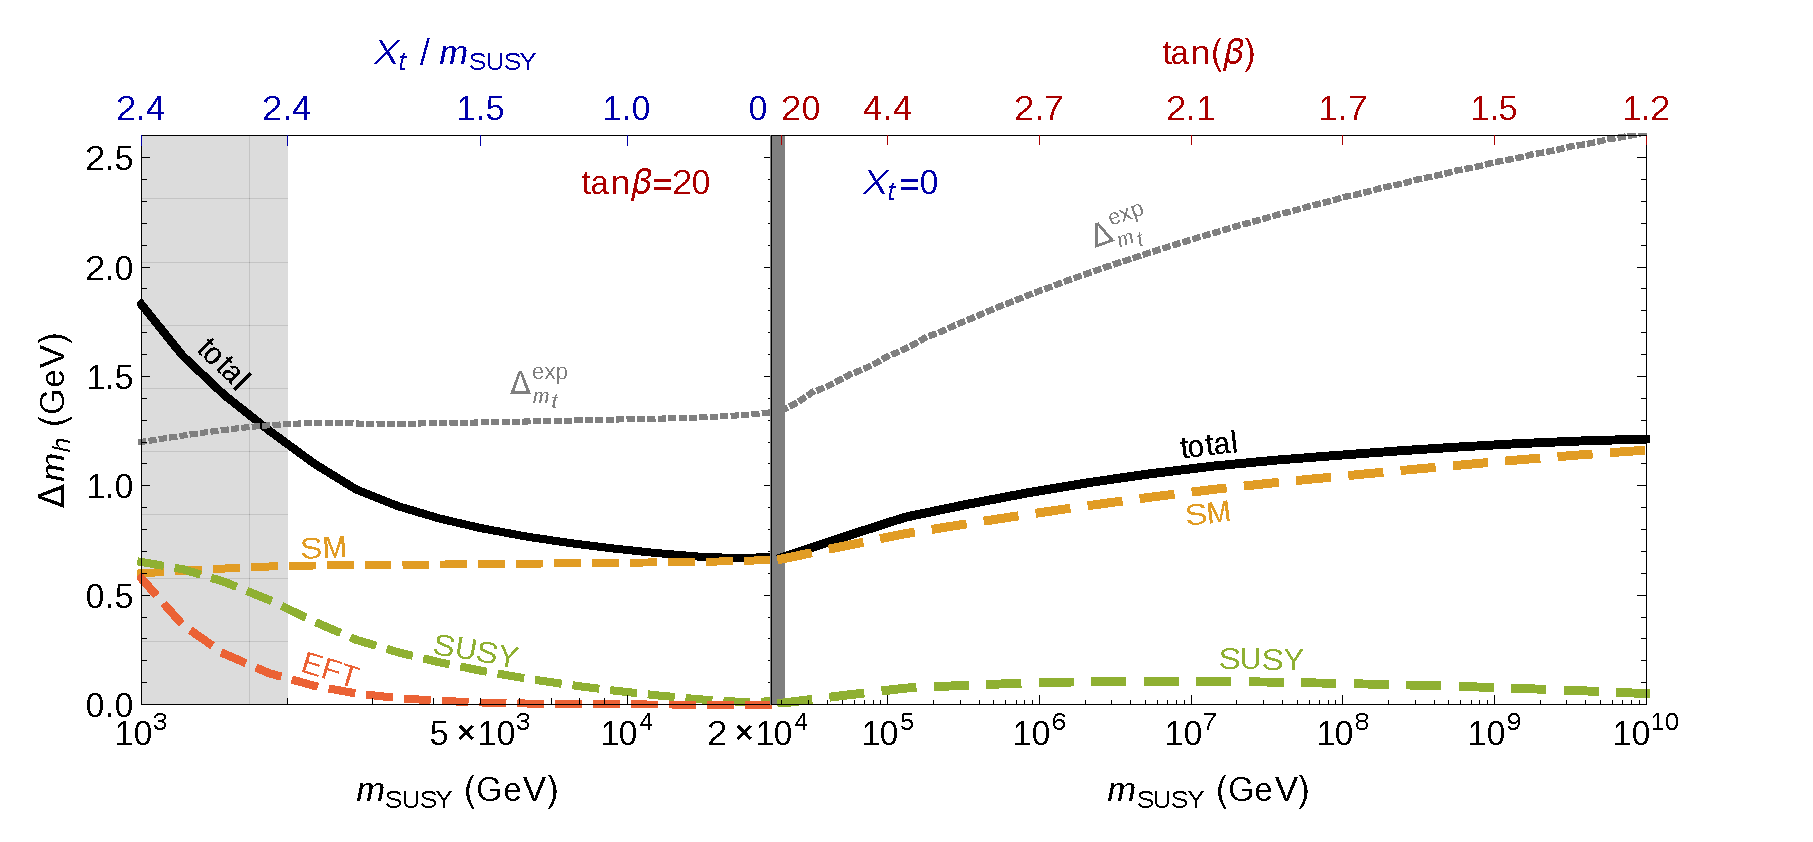
\includegraphics[width=\textwidth]{plots/kuts-10/SUSYHD-uncertainties}
  \end{center}
  \flushright Image taken from \bigcite{1504.05200}
\end{frame}

\begin{frame}{Motivation --- SM uncertainty in \HSSUSY}
  \begin{center}
    \includegraphics[width=0.6\textwidth]{plots/kuts-9/HSSUSY_TB-20_Xt--sqrt6_individual}
  \end{center}
  \flushright Image taken from \bigcite{1804.09410}
\end{frame}

\section{Update on the Standard Model Uncertainty}
\subsection{EFT calculation in \fs (\texttt{HSSUSY})}

%%%%%%%%%%%%%%%%%%%%%%%%%%%%%%%%%%%%%%%%
\begin{frame}{Contents}
  \tableofcontents[currentsection,currentsubsection]
\end{frame}
%%%%%%%%%%%%%%%%%%%%%%%%%%%%%%%%%%%%%%%%

\begin{frame}{EFT calculation in \fs (\texttt{HSSUSY})}
  \begin{center}
    \includegraphics[width=0.8\textwidth]{images/FS-HSSUSY.png}
  \end{center}
\end{frame}

\begin{frame}{EFT calculation in \fs (\texttt{HSSUSY})}
  \begin{center}
  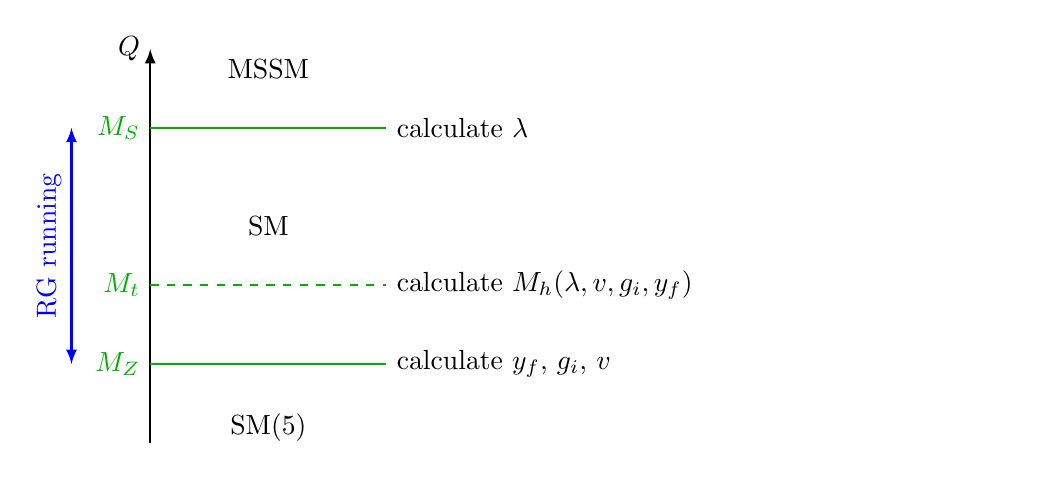
\begin{tikzpicture}
    \path[arrow] (0,0) -- (0,5) node[left]{$Q$};
    \draw[thick,darkgreen] (0,4) node[left]{$M_S$} -- node[above = 0.5cm,black]{MSSM} (3,4) node[right,black,text width=8cm]{calculate $\lambda$};
    \draw[thick,dashed,darkgreen] (0,2) node[left]{$M_t$} -- (3,2) node[right,black,text width=8cm]{calculate $M_h(\lambda, v, g_i, y_f)$};
    \draw[thick,darkgreen] (0,1) node[left]{$M_Z$} -- node[above = 1.5cm,black]{SM} node[below = 0.5cm,black]{SM(5)} (3,1) node[right,black,text width=8cm]{
      calculate $y_f$, $g_i$, $v$};
    \path[arrow,latex-latex,blue] (-1,1) -- node[above,rotate=90]{RG running} (-1,4);
  \end{tikzpicture}
  \end{center}
\end{frame}

\begin{frame}{EFT calculation in \fs (\texttt{HSSUSY})}
  \centering
  \begin{tabular}{llllll}
    \toprule
               & 1\Loop & 2\Loop & 3\Loop & 4\Loop & 5\Loop\\
    \midrule
    $\lambda$  & full & $(\at+\ab)\as$, & $\at\as^2$ & -- & -- \\
               &      & $(\at+\ab)^2$, \\
               &      & $\ab\atau$, $\atau^2$ \\
    $v$        & full & -- & -- & -- & -- \\
    $y_t$      & full & $\as^2$, \textcolor{red}{$\at\as$}, \textcolor{red}{$\at^2$} & $\as^3$ & $\textcolor{red}{\as^4}$ & -- \\
    $y_{b,\tau}$ & full & -- & -- & -- & -- \\
    $g_3$      & full & $\as^2$ &  $\as^3$ & -- & -- \\
    $g_{1,2}$   & full & -- & -- & -- & -- \\
    \midrule
    $\beta_{\lambda}$ & full & full & full & $\at^2\as^3$ & -- \\
    $\beta_{y_t}$    & full & full & full & $y_t\as^4$ & -- \\
    $\beta_{g_3}$    & full & full & full & $\as^{0<n\le 4}$ & $\as^5$ \\
    $\beta_{\cdots}$  & full & full & full & -- & -- \\
    \midrule
    $M_h$           & full & $(\at+\ab)\as$, & $\at\as^2$, \textcolor{orange}{$\at^2\as$}, \textcolor{orange}{$\at^3$} & $\at\as^3$ & -- \\
                    &      & $(\at + \ab)^2$ \\
    \bottomrule
  \end{tabular}
\end{frame}

\begin{frame}{Uncertainty estimate of the EFT calculation}
  \bigcite{1804.09410} considered 5 sources of uncertainty:
  \begin{align*}
    \textcolor{darkgreen}{\DMhQpole} &= \max_{\Qpole\in[M_t/2,2M_t]}\left|M_h(\Qpole) - M_h(M_t)\right| & \text{\mycite{1609.00371}} \\
    \DMhQmatch &= \max_{\Qmatch\in[\MS/2,2\MS]}\left|M_h(\Qmatch) - M_h(\MS)\right| & \text{\mycite{1407.4081}} \\
    \textcolor{darkgreen}{\DMhHSSUSYytSM} &= \left| M_h(y_t^{\SM,2\Loop}(M_Z)) - M_h(y_t^{\SM,3\Loop}(M_Z)) \right| & \text{\mycite{1504.05200}} \\
    \DMhEFT &= \left| M_h - M_h(v^2/\MS^2) \right| & \text{\mycite{1504.05200}} \\
    \DMhHSSUSYytMSSM &= \left| M_h - M_h(y_t^\MSSM(\MS)) \right| & \text{\mycite{Bagnaschi,AV,Weiglein}}
  \end{align*}
  Combination:
  \begin{align*}
    \DMhHSSUSY &= \DMhQpole + \DMhQmatch + \DMhHSSUSYytSM + \DMhHSSUSYytMSSM \\
    &\quad + \DMhEFT
  \end{align*}
\end{frame}

\begin{frame}{Uncertainty estimate of the EFT calculation}
  \begin{center}
    \includegraphics[width=0.7\textwidth]{plots/kuts-9/HSSUSY_TB-20_Xt--sqrt6_individual}
  \end{center}
\end{frame}

\subsection{Adding $O(\at\as, \at^2)$ and $O(\as^4)$ corrections to $m_t$}

%%%%%%%%%%%%%%%%%%%%%%%%%%%%%%%%%%%%%%%%
\begin{frame}{Contents}
  \tableofcontents[currentsection,currentsubsection]
\end{frame}
%%%%%%%%%%%%%%%%%%%%%%%%%%%%%%%%%%%%%%%%

\begin{frame}{Adding $O(\at\as, \at^2)$ and $O(\as^4)$ corrections to $m_t$}
  Adding 2-loop corrections of $O(\at\as, \at^2)$ \bigcite{1604.01134}
  and $O(\as^4)$ \bigcite{1508.00912}:
\begin{align*}
  m_t &= M_t
  + \Sigma_{S,\text{non-QCD}}^{(1\Loop)}
  + \textcolor{red}{\Sigma_{S,\at\as}^{(2\Loop)}}
  + \textcolor{red}{\Sigma_{S,\at^2}^{(2\Loop)}} \\
  &\phantom{={}} + M_t \Big[ \Sigma_{L,\text{non-QCD}}^{(1\Loop)} + \Sigma_{R,\text{non-QCD}}^{(1\Loop)}
    + \Delta m_{\as}^{(1\Loop)} \\
  &\phantom{={} + M_t \Big[}
    + \Delta m_{\as^2}^{(2\Loop)}
    + \textcolor{red}{\Delta m_{\at\as}^{(2\Loop)}}
    + \textcolor{red}{\Delta m_{\at^2}^{(2\Loop)}} \\
  &\phantom{={} + M_t \Big[}
    + \Delta m_{\as^3}^{(3\Loop)}
    + \textcolor{red}{\Delta m_{\as^4}^{(4\Loop)}}
  \Big]
\end{align*}
at $p^2 = M_t^2$ and  $Q = M_Z$.
\end{frame}

\begin{frame}{Effect of 2\Loop corrections to $m_t$ on $M_h$}
  \begin{center}
    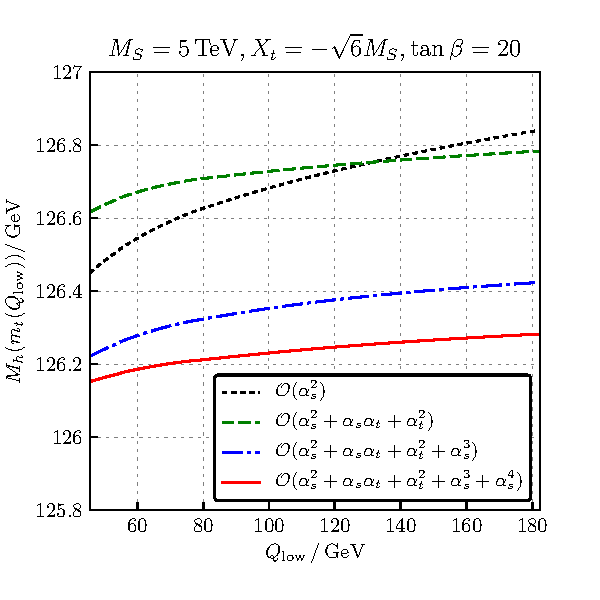
\includegraphics[width=0.5\textwidth]{plots/kuts-10/Mh_Qlow_mt_2L_3LQCD_4LQCD}\hfill
    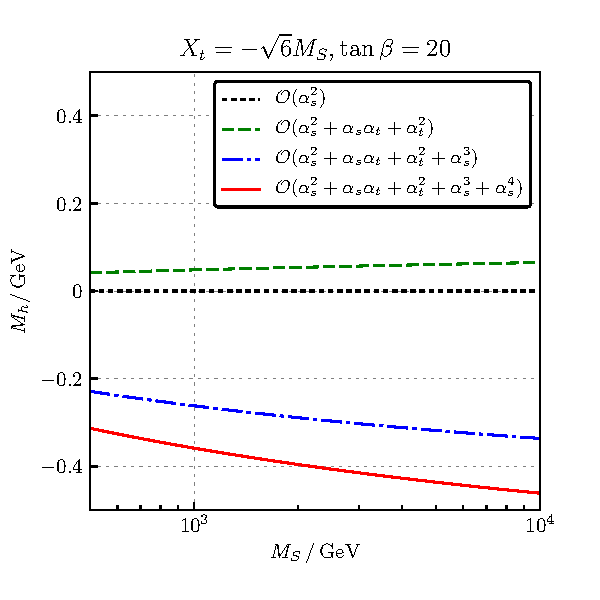
\includegraphics[width=0.5\textwidth]{plots/kuts-10/DMh_MS_mt_2L_3LQCD_4LQCD}
  \end{center}
\end{frame}

\begin{frame}{Intermediate conclusions}
  In the shown parameter region ($X_t = -\sqrt{6}M_S$, $\tan\beta = 20$)
  \begin{itemize}
  \item 2-loop $O(\at\as, \at^2)$ corrections are $\lesssim 80\MeV$
  \item 3-loop $O(\at^3)$ corrections are $\lesssim 400\MeV$
  \item 4-loop $O(\at^4)$ corrections are $\lesssim 130\MeV$
  \end{itemize}
  \vspace*{0.5em}
  $\Rightarrow$ The uncertainty estimate \bigcite{1504.05200}
  \begin{align*}
    \DMhHSSUSYytSM &= \left| M_h(y_t^{\SM,2\Loop}(M_Z)) - M_h(y_t^{\SM,3\Loop}(M_Z)) \right| \sim 400\MeV
  \end{align*}
  captures the main effect of missing 4-loop corrections to $M_h$.
\end{frame}

\subsection{Update of the SM uncertainty}

%%%%%%%%%%%%%%%%%%%%%%%%%%%%%%%%%%%%%%%%
\begin{frame}{Contents}
  \tableofcontents[currentsection,currentsubsection]
\end{frame}
%%%%%%%%%%%%%%%%%%%%%%%%%%%%%%%%%%%%%%%%

\begin{frame}{Update of SM uncertainty}
  \centering
  \begin{tabular}{llllll}
    \toprule
               & 1\Loop & 2\Loop & 3\Loop & 4\Loop & 5\Loop\\
    \midrule
    $\lambda$  & full & $(\at+\ab)\as$, & $\at\as^2$ & -- & -- \\
               &      & $(\at+\ab)^2$, \\
               &      & $\ab\atau$, $\atau^2$ \\
    $v$        & full & -- & -- & -- & -- \\
    $y_t$      & full & $\as^2$, \textcolor{darkgreen}{$\at\as$}, \textcolor{darkgreen}{$\at^2$} & $\as^3$ & $\textcolor{orange}{\as^4}$ & -- \\
    $y_{b,\tau}$ & full & -- & -- & -- & -- \\
    $g_3$      & full & $\as^2$ &  $\as^3$ & -- & -- \\
    $g_{1,2}$   & full & -- & -- & -- & -- \\
    \midrule
    $\beta_{\lambda}$ & full & full & full & $\at^2\as^3$ & -- \\
    $\beta_{y_t}$    & full & full & full & $y_t\as^4$ & -- \\
    $\beta_{g_3}$    & full & full & full & $\as^{0<n\le 4}$ & $\as^5$ \\
    $\beta_{\cdots}$  & full & full & full & -- & -- \\
    \midrule
    $M_h$           & full & $(\at+\ab)\as$, & $\at\as^2$, \textcolor{darkgreen}{$\at^2\as$}, \textcolor{darkgreen}{$\at^3$} & $\at\as^3$ & -- \\
                    &      & $(\at + \ab)^2$ \\
    \bottomrule
  \end{tabular}
\end{frame}

\begin{frame}{Update of SM uncertainty}
  Updated SM uncertainty:
  \begin{align*}
    \DMhQpole &= \max_{\Qpole\in[M_t/2,2M_t]}\left|M_h(\Qpole) - M_h(M_t)\right| \\
    \DMhHSSUSYytSM &= \left| M_h(y_t^{\SM,\textcolor{red}{3\Loop}}(M_Z)) - M_h(y_t^{\SM,\textcolor{red}{4L}}(M_Z)) \right|
  \end{align*}
\end{frame}

\begin{frame}{Update of SM uncertainty}
  \begin{columns}
    \begin{column}{0.5\textwidth}
      \centering
      \bigcite{1804.09410}\\
      \includegraphics[width=\textwidth]{plots/kuts-9/HSSUSY_TB-20_Xt--sqrt6_individual}\\
      $\MS(M_h^{\text{exp}}) \approx 3.45\TeV$\\
      $\Delta M_h \approx 1.0\GeV$
    \end{column}
    \begin{column}{0.5\textwidth}
      \centering
      This talk\\
      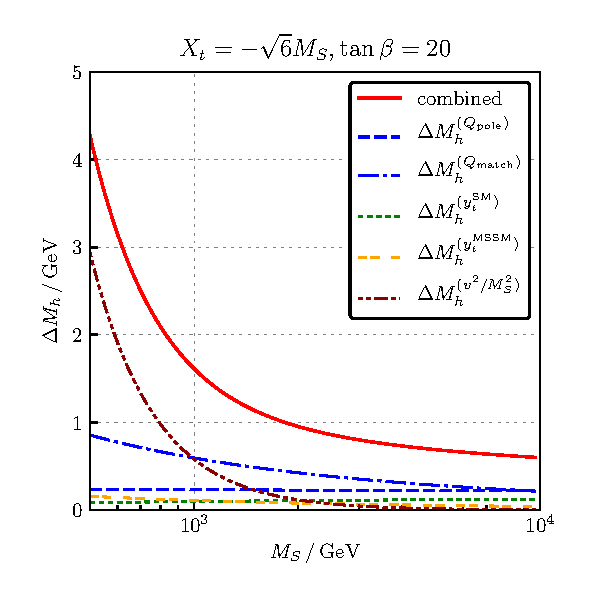
\includegraphics[width=\textwidth]{plots/kuts-10/DMh_MS_individual}\\
      $\MS(M_h^{\text{exp}}) \approx 3.50\TeV$\\
      $\Delta M_h \approx 0.75\GeV$
    \end{column}
  \end{columns}
\end{frame}

\section{When should the EFT be used?}

%%%%%%%%%%%%%%%%%%%%%%%%%%%%%%%%%%%%%%%%
\begin{frame}{Contents}
  \tableofcontents[currentsection]
\end{frame}
%%%%%%%%%%%%%%%%%%%%%%%%%%%%%%%%%%%%%%%%

\begin{frame}{When should the EFT be used?}
  \begin{columns}
    \begin{column}{0.5\textwidth}
      \centering
      \bigcite{1804.09410}\\
      \includegraphics[width=\textwidth]{plots/kuts-9/Mh_MS_TB-20_Xt--sqrt6}\\
      $\DMh \overset{!}{=} \DMhHSSUSY$\\[0.5em]
      $\Rightarrow$ $\MS^{\text{equal}} = 1.0$--$1.3\TeV$
    \end{column}
    \begin{column}{0.5\textwidth}
      \centering
      This talk\\
      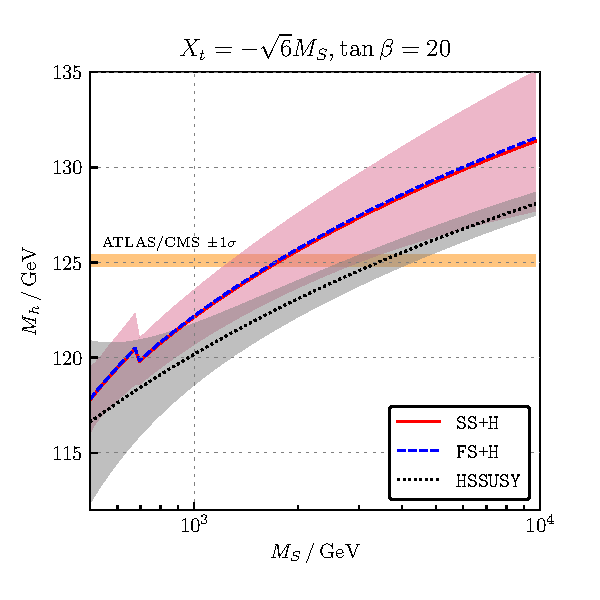
\includegraphics[width=\textwidth]{plots/kuts-10/DMh_MS_combined}\\
      $\DMh \overset{!}{=} \DMhHSSUSY$\\[0.5em]
      $\Rightarrow$ $\MS^{\text{equal}} = 1.0$--$1.2\TeV$
    \end{column}
  \end{columns}
\end{frame}

\begin{frame}[noframenumbering]
  \begin{center}
    \Huge Backup
  \end{center}
\end{frame}

\begin{frame}[noframenumbering]{References for loop corrections used in \HSSUSY}
  $\lambda$: \mycite{1407.4081, 1504.05200, 1703.08166, 1807.03509}\\
  $M_h$: \mycite{1205.6497, 1504.05200, 1407.4336, 1508.00912}\\
  $y_t$: \mycite{9911434, 9912391, 1604.01134}\\
  $g_3$: \mycite{9305305, 9707474, 9708255, 0004189}\\
  $\beta_i$: \mycite{1201.5868, 1210.6873, 1212.6829, 1205.2892, 1303.4364, 1508.00912, 1508.02680, 1604.00853, 1606.08659}
\end{frame}

\begin{frame}[noframenumbering]{Uncertainty estimate of the fixed-order calculation}
  \bigcite{1804.09410} considered 5 sources of uncertainty:
  \begin{align*}
    \DMhQpole &= \max_{\Qpole\in[\MS/2,2\MS]}\left|M_h(\Qpole) - M_h(\MS)\right| & \text{\mycite{1609.00371}} \\
    \DMhQmatch &= \max_{\Qmatch\in[M_Z/2,2M_Z]}\left|M_h(\Qmatch) - M_h(M_Z)\right| & \text{\mycite{1804.09410}} \\
    \DMhMt &= \left|M_h(m_t^{(1)}) - M_h(m_t^{(2)})\right| & \text{\mycite{1609.00371}} \\
    \DMhAlphaS &= \left| M_h(\as^{(1)}) - M_h(\as^{(2)}) \right| & \text{\mycite{1804.09410}} \\
    \DMhAlphaEm &= \left| M_h(\aem^{(1)}) - M_h(\aem^{(2)}) \right| & \text{\mycite{1804.09410}}
  \end{align*}
  Combination:
  \begin{align*}
    \DMh &= \DMhQpole + \DMhQmatch + \DMhMt + \DMhAlphaS + \DMhAlphaEm 
  \end{align*}
\end{frame}

\end{document}
